\section{Introduction}

Capturing section of the screen might seems a simple tasks, but it is often hidden away behind lesser known shortcuts or small apps and not necessarily commonly known. We tried to use the voice to help with such task.

\section{Outline}

By bringing the voice to help us with the task, we're not trying to be necessarily faster than using the different options already there, but we're focusing on adding a vocal to different small tasks to complement the standard usage in a connected world.
Inspired by different solutions used to take screenshots, our concept is relatively straight forward: the user will speak a command to start the selection, drag their mouse over a portion of their screen and then speak a second command word to have it capture.

\subsection{CASE/CARE}
\begin{figure}
    \centering
    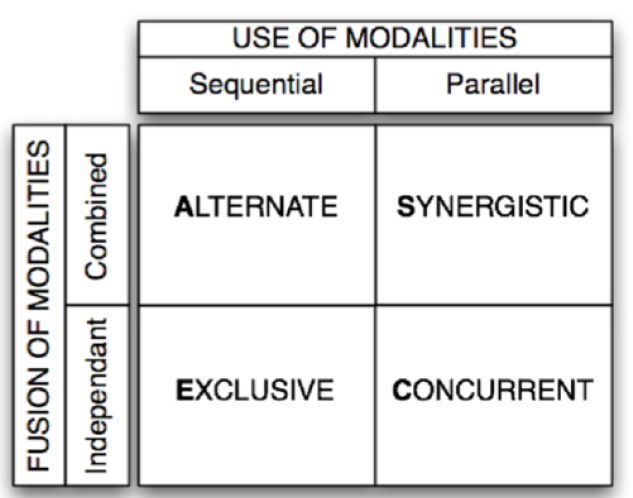
\includegraphics[scale=.6]{Report/images/CaseCare.png}
    \caption{CASE model}
    \label{fig:my_label}
\end{figure}

The utility will require them to use mouse, keyboard and voice in a \textbf{synergistic fashion} in the CASE model.
The position of the mouse is grabbed as the voice command is activated.

For the user, both applications are used \textbf{complimentary}.
As the mouse position will define the section selected when the words are spoken. 

\section{Architecture}
We went with Python for its strength in quick prototyping, good turnaround, extensive library and tools available across and our personal skills and knowledge.
Which turned out to be really helpful.

\subsection{Implementation}
\subsubsection*{Voice recognition}
The main part of the project is obviously the voice.
For this aspect, we used the speech recognition package with the Google Cloud Speech API.
The speech recognition listen for some audio input from the user and then convert it to text. Once we have the text, we can seek for keywords to then execute the rest of the code.
In our case we put this speech recognition in a while loop to  to have the two position of the mouse that we needed for the rest of the program.

\subsubsection*{Screen capture}
Capturing the section of the screen turned out to be fast and direct. Thanks to a library called PIL (more specifically a forked named Pillow) capturing a screenshot is a couple of lines of codes. 

%\lstinputlisting[language=python, firstline = 150, lastline = 159]{../voicegrab.py}

\subsubsection*{Comfort and feedback}
[K]

\subsection{In the utility}


\section{User test and data analysis}
Due to the peculiar times we are living, we had only four users for this test. This is why we chose to do the "within group" method.
Our four users had to fill a google form asking some questions to have information about them, what part of the population the were, what they usually do to take screenshots, etc.


\section{Conclusion}

During this project we hit a few hiccup and limitations making our utility less effective. The voice recognition is slow, which makes the usage of it slightly awkward. While slow the Speech-To-Text solution is quite powerful. 

\subsection*{Improvement paths}
The 